\documentclass{article}

% if you need to pass options to natbib, use, e.g.:
%     \PassOptionsToPackage{numbers, compress}{natbib}
% before loading neurips_2025

% The authors should use one of these tracks.
% Before accepting by the NeurIPS conference, select one of the options below.
% 0. "default" for submission
 \usepackage[preprint]{neurips_2025}
% the "default" option is equal to the "main" option, which is used for the Main Track with double-blind reviewing.
% 1. "main" option is used for the Main Track
%  \usepackage[main]{neurips_2025}
% 2. "position" option is used for the Position Paper Track
%  \usepackage[position]{neurips_2025}
% 3. "dandb" option is used for the Datasets & Benchmarks Track
 % \usepackage[dandb]{neurips_2025}
% 4. "creativeai" option is used for the Creative AI Track
%  \usepackage[creativeai]{neurips_2025}
% 5. "sglblindworkshop" option is used for the Workshop with single-blind reviewing
 % \usepackage[sglblindworkshop]{neurips_2025}
% 6. "dblblindworkshop" option is used for the Workshop with double-blind reviewing
%  \usepackage[dblblindworkshop]{neurips_2025}

% After being accepted, the authors should add "final" behind the track to compile a camera-ready version.
% 1. Main Track
 % \usepackage[main, final]{neurips_2025}
% 2. Position Paper Track
%  \usepackage[position, final]{neurips_2025}
% 3. Datasets & Benchmarks Track
 % \usepackage[dandb, final]{neurips_2025}
% 4. Creative AI Track
%  \usepackage[creativeai, final]{neurips_2025}
% 5. Workshop with single-blind reviewing
%  \usepackage[sglblindworkshop, final]{neurips_2025}
% 6. Workshop with double-blind reviewing
%  \usepackage[dblblindworkshop, final]{neurips_2025}
% Note. For the workshop paper template, both \title{} and \workshoptitle{} are required, with the former indicating the paper title shown in the title and the latter indicating the workshop title displayed in the footnote.
% For workshops (5., 6.), the authors should add the name of the workshop, "\workshoptitle" command is used to set the workshop title.
% \workshoptitle{WORKSHOP TITLE}

% "preprint" option is used for arXiv or other preprint submissions
 % \usepackage[preprint]{neurips_2025}

% to avoid loading the natbib package, add option nonatbib:
%    \usepackage[nonatbib]{neurips_2025}

\usepackage[utf8]{inputenc} % allow utf-8 input
\usepackage[T1]{fontenc}    % use 8-bit T1 fonts
\usepackage{hyperref}       % hyperlinks
\usepackage{url}            % simple URL typesetting
\usepackage{booktabs}       % professional-quality tables
\usepackage{amsfonts}       % blackboard math symbols
\usepackage{nicefrac}       % compact symbols for 1/2, etc.
\usepackage{microtype}      % microtypography
\usepackage{xcolor}         % colors
\usepackage{graphicx}
\usepackage{amsmath}
\usepackage{CJKutf8}
% Note. For the workshop paper template, both \title{} and \workshoptitle{} are required, with the former indicating the paper title shown in the title and the latter indicating the workshop title displayed in the footnote. 
\title{Uncertainty-Aware KV Cache Compression for Training-Free Efficient Language Model Inference}


% The \author macro works with any number of authors. There are two commands
% used to separate the names and addresses of multiple authors: \And and \AND.
%
% Using \And between authors leaves it to LaTeX to determine where to break the
% lines. Using \AND forces a line break at that point. So, if LaTeX puts 3 of 4
% authors names on the first line, and the last on the second line, try using
% \AND instead of \And before the third author name.


\begin{document}


\begin{CJK*}{UTF8}{gbsn}
\author{%
  范文茜 \\
  524531910002 \\
  \And
  裘嘉敏 \\
  524030910068 \\
  \And
  陆紫萌 \\
  524531910001 \\
}
\maketitle
\end{CJK*}


\begin{abstract}
  The KV cache compression during
  transformer inference can be unreliable when token
  importance differs across KV heads. We propose an uncertainty-aware wrapper
  for score-based KVPress methods that augments each token's average importance
  with a head-wise variance term, allowing the compressor to preserve tokens
  whose relevance is uncertain across heads. The method is training-free,
  simple to implement, and compatible with multiple existing presses. Experiments
  on Pythia-70m using WikiText-2 and PG-19 show that the uncertainty term
  substantially improves KNorm compression, reducing WikiText-2 perplexity from
  50.52 to 42.46 at a 0.5 compression ratio, while providing limited or negative
  gains for stronger base presses such as SnapKV, CUR, and LagKV. These results
  suggest that head-wise disagreement is a useful correction signal for simple
  static scoring methods, but its benefit depends on the base compression
  mechanism.
\end{abstract}


\section{Introduction}

Key-Value (KV) cache compression is a practical training-free approach for transformer optimization. However, a token with moderate average importance but large head-wise disagreement may still be risky to prune, because some heads may rely on it strongly. Motivated by the observation that token importance is not always
  agreed upon across KV heads~\citep{ICLR2024_639a9a17}, we propose an uncertainty-aware KV cache compression wrapper for score-based presses in KVPress.It reuses a base scorer and augments its token ranking with a head-disagreement term. Given per-head token scores, we compute the mean importance across heads and the variance across heads, then rank tokens by
  \[
      s_i = \operatorname{Norm}\!\left(\mathbb{E}_{h}[s_{h,i}]\right)
      + \lambda \operatorname{Norm}\!\left(\operatorname{Var}_{h}
  [s_{h,i}]\right),
  \]
  where $\lambda$ controls the degree of risk aversion. This design is simple, training-free, and compatible with multiple existing score-based KV compression methods. Intuitively, the method keeps tokens that are either consistently important across heads or uncertain because different heads assign them very different scores. 

\section{Method}

  We propose an uncertainty-aware KV cache compression method that
  wraps an existing score-based KVPress and accounts for disagreement between KV heads when estimating token importance. Instead of pruning only by the base importance
  score, we augment the score with an uncertainty term estimated from inter-head variance.

  Let the base press produce token scores
  \[
  S \in \mathbb{R}^{B \times H \times L},
  \]
  where \(B\) is the batch size, \(H\) is the number of KV heads, and \(L\) is the sequence length. These
  scores can come from different base methods. For each token position \(t\), we compute the mean score across KV heads:
  \[
  \mu_t = \mathrm{mean}_{h}(S_{h,t}),
  \]
  and define the uncertainty term as the head-wise variance of the base scores:
  \[
  u_t = \mathrm{Var}_{h}(S_{h,t}).
  \]

  The adjusted token score is then
  \[
  a_t = \mathrm{norm}(\mu_t) + \lambda \cdot \mathrm{norm}(u_t),
  \]
  where \(\lambda\) is the uncertainty weight. A larger \(\lambda\) makes the compressor more conservative toward tokens
  whose importance is uncertain across heads. In the implementation, both the mean score and the uncertainty term are
  min--max normalized along the sequence dimension, with a small \(\epsilon\) for numerical stability. This makes the
  combination less sensitive to the raw score scale of different base presses.

  After computing the adjusted score, the same token-level score is expanded back to all KV heads. The standard
  \texttt{ScorerPress} compression mechanism is then used: for a target compression ratio, the method keeps the top-scoring KV positions and removes the lowest-scoring ones during prefill.

\section{Experiments}  \label{sec:experiments}

We evaluate whether the proposed uncertainty-aware score adjustment improves KV cache compression under different base presses. 
Our experiments focus on three questions:
(i) whether uncertainty-aware adjustment reduces perplexity under the same compression ratio;
(ii) whether the improvement is consistent across different scoring mechanisms;
and (iii) whether the additional scoring computation affects inference efficiency.

\begin{figure}[!htbp]
    \centering
    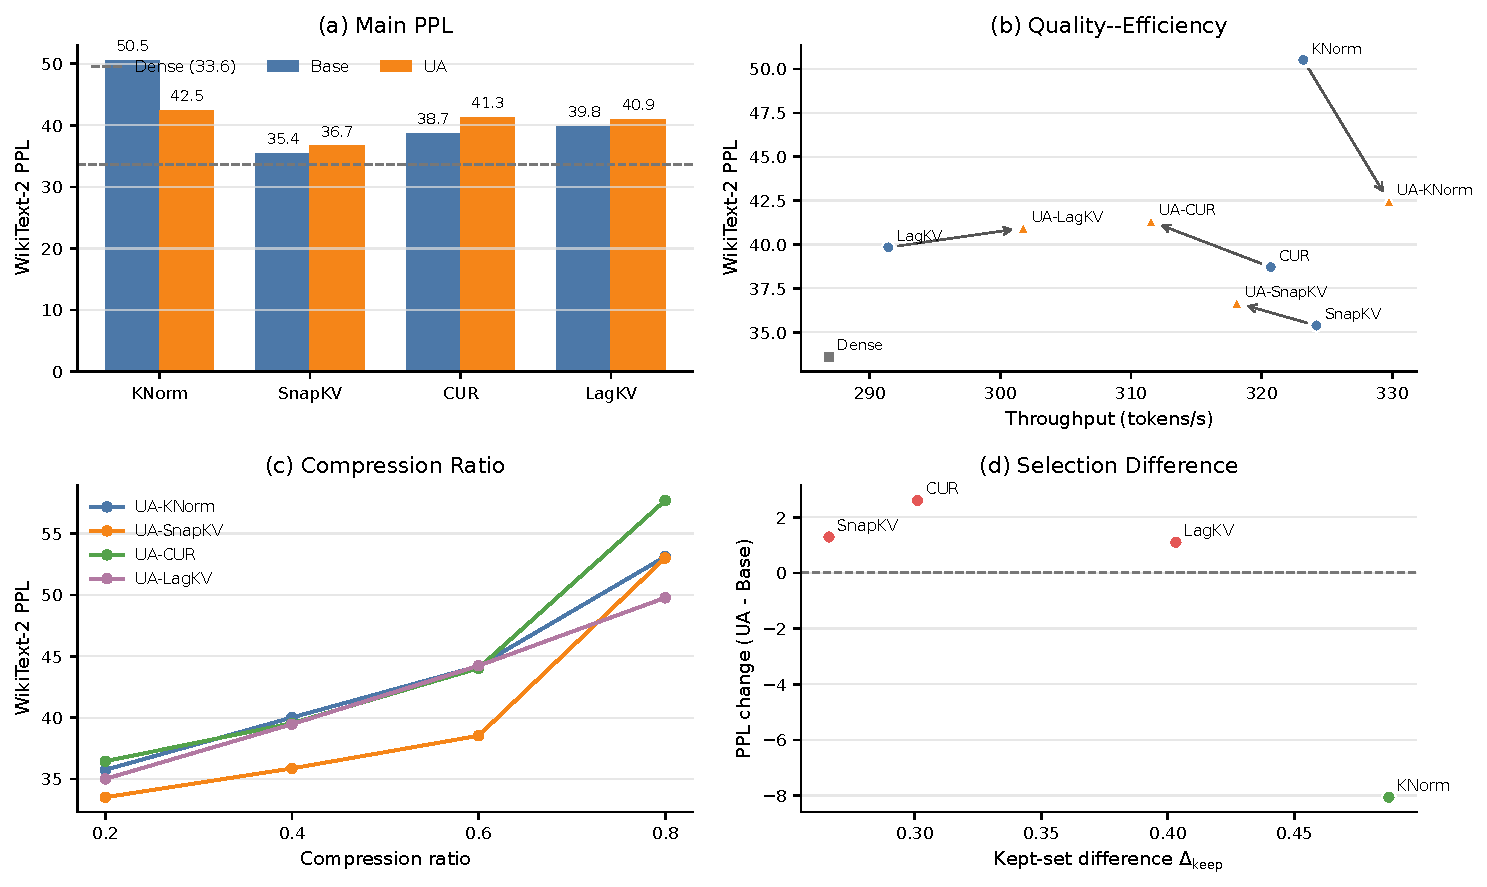
\includegraphics[width=1\linewidth]{ua_press_summary.pdf}
    \caption{
Experimental summary of uncertainty-aware KV cache compression.
(a) Main perplexity comparison between base presses and their uncertainty-aware variants.
(b) Quality-efficiency trade-off measured by perplexity and throughput.
(c) Perplexity under different compression ratios.
(d) Retained-token set difference versus perplexity change, where negative PPL change indicates improvement.
}
    \label{experiment_summary}
\end{figure}


\subsection{Experimental Setup}

\textbf{Model.} All experiments are conducted on \texttt{EleutherAI/pythia-70m}. We use the same model checkpoint for all methods to ensure a controlled comparison. \textbf{Datasets.} We evaluate language modeling quality on WikiText-2 and PG-19. WikiText-2 is used as the primary benchmark for perplexity evaluation, while PG-19 is used to test long-context behavior. \textbf{Compared methods.} The original kvpress methods we apply include \texttt{KNorm}, \texttt{CURPress}, \texttt{SnapKVPress}, and \texttt{LagKVPress}. We compare these methods with their uncertainty-aware variants. We also include a dense baseline without KV cache compression. All compression methods are implemented under the \texttt{kvpress} framework. \textbf{Compute.} All experiments are conducted on a single NVIDIA GeForce RTX 4060 GPU using CUDA. \textbf{Default evaluation parameters.} Unless otherwise specified, all experiments use the same evaluation configuration shown in Table~\ref{tab:default_params}. 

\begin{table}[!htbp]
\centering
\caption{Default evaluation parameters used in our experiments.}
\label{tab:default_params}
\begin{tabular}{l c l}
\toprule
Parameter & Default Value & Description \\
\midrule
\texttt{dataset} & \texttt{wikitext-2} & Dataset dataset used for evaluation \\
\texttt{split} & \texttt{test} & Dataset split used for evaluation \\
\texttt{num-samples} & 10 & Number of evaluated samples \\
\texttt{warmup-runs} & 2 & Number of warmup runs \\
\texttt{context-tokens} & 1024 & Number of context tokens used for compression \\
\texttt{target-tokens} & 256 & Number of target tokens used for PPL evaluation \\
\texttt{max-new-tokens} & 64 & Maximum number of generated tokens for speed evaluation \\
\texttt{compression-ratio} & 0.5 & Fraction of KV cache entries removed \\
\texttt{uncertainty-weight} & 1.0 & Weight $\lambda$ for the uncertainty term \\
\bottomrule
\end{tabular}
\end{table}

\subsection{Main Results}
\label{subsec:main_results}

Table~\ref{tab:main_results} reports the main results under the default compression ratio $r=0.5$.
Compared with vanilla \texttt{KNorm}, \texttt{UA-KNorm} reduces WikiText-2 perplexity from $50.52$ to $42.46$, corresponding to a relative improvement of $15.96\%$.
However, for \texttt{SnapKV}, \texttt{CUR}, and \texttt{LagKV}, the uncertainty-aware variants do not improve perplexity under the default setting.

In terms of efficiency, the uncertainty-aware wrapper does not change the target cache size, so the decoding-time cost remains close to the corresponding base press.
This supports that the additional mean-variance computation mainly affects the scoring stage rather than the compressed decoding process.

\begin{table}[!htbp]
\centering
\caption{Main results on WikiText-2 and PG-19 under compression ratio $r=0.5$.
Lower PPL, TTFT, and TPOT are better; higher throughput is better.
TTFT and TPOT are reported in milliseconds.}
\label{tab:main_results}
\resizebox{\linewidth}{!}{
\begin{tabular}{l c c c c c c}
\toprule
Method & Ratio & WikiText-2 PPL $\downarrow$ & PG-19 PPL $\downarrow$ & TTFT (ms) $\downarrow$ & TPOT (ms) $\downarrow$ & Throughput $\uparrow$ \\
\midrule
Dense       & 0.0 & 33.61 & 32.10 & 12.85 & 3.31 & 286.90 \\
\midrule
KNorm       & 0.5 & 50.52 & 39.45 & 13.64 & 2.90 & 323.19 \\
UA-KNorm    & 0.5 & 42.46 & 33.83 & 14.69 & 2.82 & 329.74 \\
\midrule
SnapKV      & 0.5 & 35.38 & 34.10 & 16.25 & 2.85 & 324.19 \\
UA-SnapKV   & 0.5 & 36.67 & 36.28 & 17.73 & 2.88 & 318.11 \\
\midrule
CUR         & 0.5 & 38.71 & 37.57 & 14.96 & 2.90 & 320.70 \\
UA-CUR      & 0.5 & 41.31 & 40.71 & 17.15 & 2.96 & 311.53 \\
\midrule
LagKV       & 0.5 & 39.83 & 32.56 & 17.89 & 3.17 & 291.43 \\
UA-LagKV    & 0.5 & 40.94 & 33.09 & 17.43 & 3.06 & 301.76 \\
\bottomrule
\end{tabular}
}
\end{table}

\subsection{Effect of Compression Ratio} %Add thoughout to discuss trade-off between quality and efficiency
\label{subsec:compression_ratio} 
We further evaluate the uncertainty-aware variants under different compression ratios. Table~\ref{tab:ratio_study} shows the results.

\begin{table}[!htbp]
\centering
\caption{Perplexity and throughput on WikiText-2 under different compression ratios.
Lower PPL is better; higher throughput is better.}
\label{tab:ratio_study}
\resizebox{\linewidth}{!}{
\begin{tabular}{l c c c c c c c c}
\toprule
Method & \multicolumn{2}{c}{$r=0.2$} & \multicolumn{2}{c}{$r=0.4$} & \multicolumn{2}{c}{$r=0.6$} & \multicolumn{2}{c}{$r=0.8$} \\
\cmidrule(lr){2-3} \cmidrule(lr){4-5} \cmidrule(lr){6-7} \cmidrule(lr){8-9}
 & PPL $\downarrow$ & Throughput $\uparrow$ & PPL $\downarrow$ & Throughput $\uparrow$ & PPL $\downarrow$ & Throughput $\uparrow$ & PPL $\downarrow$ & Throughput $\uparrow$ \\
\midrule
UA-KNorm  & 35.75 & 295.11 & 40.02 & 311.80 & 44.21 & 306.06 & 53.12 & 302.56 \\
UA-SnapKV & 33.52 & 285.96 & 35.87 & 299.56 & 38.53 & 306.58 & 53.01 & 310.11 \\
UA-CUR    & 36.46 & 291.04 & 39.55 & 299.25 & 44.04 & 317.12 & 57.70 & 318.10 \\
UA-LagKV  & 35.02 & 295.04 & 39.47 & 307.41 & 44.24 & 308.62 & 49.77 & 314.59 \\
\bottomrule
\end{tabular}
}
\end{table}
As expected, throughput generally improves as the compression ratio increases, although the trend is not perfectly monotonic for every method. This is because a larger ratio removes more KV cache entries, reducing attention computation and memory access during generation. However, the same increase in ratio also worsens perplexity, so the compression ratio should be chosen as a trade-off between quality and efficiency.
\subsection{Ablation Study}
\label{subsec:ablation}

\paragraph{Effect of uncertainty weight.}
Table~\ref{tab:lambda_ablation} studies the effect of the uncertainty weight $\lambda$.
For \texttt{UA-KNorm}, adding the uncertainty term consistently improves over $\lambda=0$.
The PPL decreases from $43.13$ at $\lambda=0$ to $40.99$ at $\lambda=0.5$ and further to $40.65$ at $\lambda=2.0$.
This confirms that head-wise variance is a useful correction signal for \texttt{KNorm}.
For \texttt{UA-SnapKV}, \texttt{UA-CUR}, and \texttt{UA-LagKV}, changing $\lambda$ has little effect or slightly worsens PPL, suggesting that these methods already capture token importance through their original scores and that head-wise variance provides little, or even negative, additional signal.



\begin{table}[!htbp]
\centering
\caption{Ablation on uncertainty weight $\lambda$ on WikiText-2 under compression ratio $r=0.5$.
Lower PPL is better.}
\label{tab:lambda_ablation}
\begin{tabular}{l c c c c c}
\toprule
Method & $\lambda=0$ & $\lambda=0.25$ & $\lambda=0.5$ & $\lambda=1.0$ & $\lambda=2.0$ \\
\midrule
UA-KNorm  & 43.13 & 42.38 & 40.99 & 42.46 & 40.65 \\
UA-SnapKV & 37.03 & 37.20 & 36.94 & 36.67 & 36.65 \\
UA-CUR    & 39.63 & 40.83 & 41.96 & 41.31 & 41.13 \\
UA-LagKV  & 40.97 & 40.73 & 40.73 & 40.94 & 41.50 \\
\bottomrule
\end{tabular}
\end{table}

\paragraph{Effect of normalization.}
Table~\ref{tab:norm_ablation} evaluates the normalization choices using \texttt{UA-KNorm}.
These results show that normalization is not always beneficial for \texttt{KNorm}.
The raw score magnitude itself may already contain useful information about token importance.
Over-normalizing the score distribution may weaken this information and make the final ranking less faithful to the original key-space geometry.
Therefore, although normalization makes the method more comparable across different base presses, it may not be optimal for every individual press.

\begin{table}[!htbp]
\centering
\caption{Ablation on mean-score and variance normalization for UA-KNorm on WikiText-2.
Lower PPL is better.}
\label{tab:norm_ablation}
\begin{tabular}{l c c c}
\toprule
Variant & Normalize Mean & Normalize Variance & PPL $\downarrow$ \\
\midrule
Full UA                     & \checkmark & \checkmark & 42.46 \\
w/o mean normalization       & $\times$   & \checkmark & 42.07 \\
w/o variance normalization   & \checkmark & $\times$   & 40.91 \\
Raw combination              & $\times$   & $\times$   & 41.29 \\
\bottomrule
\end{tabular}
\end{table}

% \subsection{Selection Difference Analysis}
% \label{subsec:selection_analysis}

% To further understand when uncertainty-aware adjustment is effective, we compare the retained token sets selected by each base press and its uncertainty-aware variant.
% For \texttt{KNorm}, the kept-set difference reaches $0.487$, meaning that nearly half of the selected tokens are changed after applying uncertainty-aware adjustment.
% This large ranking change is accompanied by a substantial PPL reduction of $8.06$.
% Therefore, for \texttt{KNorm}, the uncertainty term meaningfully changes the pruning decision and corrects the weakness of the original key-norm score.
% For \texttt{SnapKV}, the kept-set difference is much smaller, only $0.266$.
% Meanwhile, PPL increases by $1.29$.
% For \texttt{CUR} and \texttt{LagKV}, the kept-set differences are $0.301$ and $0.403$, respectively, but both lead to worse PPL.

% \begin{table}[!htbp]
% \centering
% \caption{Retained-token set difference between base presses and uncertainty-aware variants on WikiText-2.
% Negative PPL change indicates improvement.}
% \label{tab:selection_diff}
% \begin{tabular}{l c c c c}
% \toprule
% Base Press & Kept-set Difference $\uparrow$ & Base PPL & UA PPL & PPL Change $\downarrow$ \\
% \midrule
% KNorm  & 0.487 & 50.52 & 42.46 & -8.06 \\
% SnapKV & 0.266 & 35.38 & 36.67 &  1.29 \\
% CUR    & 0.301 & 38.71 & 41.31 &  2.60 \\
% LagKV  & 0.403 & 39.83 & 40.94 &  1.10 \\
% \bottomrule
% \end{tabular}
% \end{table}

\subsection{Discussion}
\label{subsec:discussion}

The results show that uncertainty-aware adjustment is not uniformly effective across base presses.
The uncertainty term is most effective when the original score lacks dynamic attention information, as in \texttt{KNorm}.
For stronger base methods whose scores already encode token salience through attention patterns, matrix leverage, or lag-relative information, the head-wise variance term may introduce additional noise rather than useful correction.
Another possible reason is that \texttt{SnapKV}, \texttt{CUR}, and \texttt{LagKV} originally produce per-head token scores, so different attention heads can retain different tokens according to their own salience estimates.
After applying the uncertainty-aware wrapper, these per-head scores are reduced to a shared mean-variance token score, eliminating potentially useful differences between heads.

% \paragraph{KNorm.}
% \texttt{KNormPress} benefits most clearly from uncertainty-aware adjustment.
% Since KNorm scores tokens only by the norm of key vectors, it is a static and query-free heuristic.
% It may therefore underestimate tokens that are important to only a subset of heads.
% The variance term helps recover such head-specific tokens, explaining why \texttt{UA-KNorm} improves over vanilla \texttt{KNorm} on both WikiText-2 and PG-19.

% \paragraph{SnapKV.}
% \texttt{SnapKVPress} shows little or negative improvement.
% This happens because original SnapKV selects tokens independently for each KV head. So different KV heads can keep different tokens. This is especially important for GQA/MQA, where each KV head serves a group of query heads with potentially different attention patterns. In contrast, \texttt{UncertaintyAwarePress} first averages and computes variance across KV heads, then it expands the same adjusted scores back to all heads. Some heads may lose tokens that are important specifically to them, while tokens useful only to a few heads are kept across all heads. 
% \texttt{SnapKV} already computes token importance from recent attention patterns, and the subsequent averaging and pooling operations make the scoredistribution relatively stable.
% As a result, head-wise variance provides little additional signal.

% \paragraph{CUR.}
% \texttt{CURPress} shows improvement on PG-19 but degradation on WikiText-2.
% The reason may be the possible discard of sink tokens in \texttt{UncertaintyAwareness}. \texttt{CURPress} sets the first few sink tokens to a high score:
% \texttt{scores[:, :, : self.num\_sinks] = 1.0}. But in \texttt{UncertaintyAwarePress}, the final score adds head-wise variance. Since sink tokens have the same score across heads, their variance is zero. Non-sink tokens with
%   large head disagreement can receive a higher uncertainty bonus and may outrank the sink tokens. As a result, some sink tokens may be pruned, which breaks CUR’s intended sink preservation and can hurt performance.

% \paragraph{LagKV.}
%  \texttt{LagKVPress} also shows little or negative improvement. One possible reason is that it ranks scores within each block by default:
%   \texttt{score = score.argsort(dim=-1).argsort(dim=-1) / self.lag\_size}.
%   As a result, the original score magnitudes are discarded. The score distributions across heads are therefore normalized into similar discrete rank patterns. Consequently, head-wise variance computed afterward mainly reflects differences
%   in block-wise token rankings across heads, rather than true model uncertainty.

% \paragraph{Summary.}
% Overall, uncertainty-aware adjustment is most useful for simple, static, and under-informative base scores.
% It is less useful when the base press already captures token salience through attention or structural scoring.
% Therefore, head-wise variance should be viewed as a compatibility-dependent correction signal rather than a universally reliable importance measure.

\begin{thebibliography}{1}
\small

\bibitem[Ge et~al.(2024)Ge, Zhang, Liu, Zhang, Han, and Gao]{ICLR2024_639a9a17}
Suyu Ge, Yunan Zhang, Liyuan Liu, Minjia Zhang, Jiawei Han, and Jianfeng Gao.
\newblock Model tells you what to discard: Adaptive KV cache compression for LLMs.
\newblock In B.~Kim, Y.~Yue, S.~Chaudhuri, K.~Fragkiadaki, M.~Khan, and Y.~Sun, editors,
{\it International Conference on Learning Representations}, volume 2024,
pp.\ 22975--22988, 2024.
\newblock URL \url{https://proceedings.iclr.cc/paper_files/paper/2024/file/639a9a172c044fbb64175b5fad42e9a5-Paper-Conference.pdf}.

\end{thebibliography}

\appendix
  \section{Contribution Statement}

  The work was completed collaboratively by all group members. Fan Wenqian was responsible for the implementation of the uncertainty-aware KV cache compression method and writing the method description. Qiu Jiamin was responsible for running experiments, collecting results, and analyzing the data. Lu Zimeng was responsible for writing and revising the report, including the introduction, method description, and discussion. All members participated in literature review, result analysis, and final proofreading.

\end{document}
